\section{Lasso Regression} 

  Now supposed that $d > n$, then the first problem is that we can no longer use least squares since $X^T X$ is no longer invertible and the same problem happens with maximum likelihood. This is known as the \textbf{high dimensional} or \textbf{large $p$, small $n$} problem. The most straightforward way is simply to reduce the covariates to a dimension smaller than $n$. This can be done with three ways. 
  \begin{enumerate}
    \item We perform PCA on the $X$ and use the first $k$ principal components where $k < n$. 
    \item We cluster the covariates based on their correlation. We can use one feature from each cluster or take the average of the covariates within each cluster. 
    \item We can screen the variables by choosing the $k$ features that have the largest correlation with $Y$. 
  \end{enumerate}
  Once this is done, we are back in the low dimensional regime and can use least squares. Essentially, this is a way to find a good subset of the covariates, which can be formalized by the following. Let $S$ be a subset of $[d]$ and let $X_S = (X_j \,:\, j \in S)$. If the size of $S$ is not too large, we can regress $Y$ on $X_S$ instead of $X$. 

  \begin{definition}[Best Subset Regression]
    Fix $k < d$ and let $\mathcal{S}_k$ denote all subsets of size $k$. For a given $S \in \mathcal{S}_k$, let $\beta_S$ be the best linear predictor for the subset $S$. We want to find the best subset $S$ that minimizes the loss 
    \begin{equation}
      \mathbb{E} [ (Y - \beta_S^T X_S)^2] 
    \end{equation}
    which is equivalent to finding 
    \begin{equation}
      \argmin_{\beta} \mathbb{E} [ (Y - \beta^T X)^2] \text{ subject to } ||\beta||_0 \leq k
    \end{equation}
    where $||\beta||_0$ is the number of non-zero entries in $\beta$. 
  \end{definition}

  There will be a bias variance tradeoff. As $k$ increases, the bias decreases but the variance increases. We can approximate the risk with the training error, but the minimization is over all subset of size $k$, and so this is NP-hard. Therefore, best subset regression is infeasible, but we can approximate best subset regression in two different ways. 
  \begin{enumerate}
    \item A greedy approximation leads to \textit{forward stepwise regression}. 
    \item A convex relaxation of the problem leads to the \textit{LASSO} regression. 
  \end{enumerate}
  It turns out that the theoretical guarantees and computational time for both are the same, but the Lasso is much more popular. It may be due to a cleaner form or that it's easier to study, but who knows. 

\subsection{Forward Stepwise Regression} 

  Forward stepwise regression is a greedy algorithm that starts with an empty set of covariates and adds the covariate that most improves the fit. It avoids the NP-hardness of the best subset regression by adding covariates one by one. 

  \begin{definition}[Greedy Forward Stepwise Regression]
    Given your data $\mathcal{D}$, let's first standardize it to have mean $0$ and variance $1$.\footnote{This may or may not be a good idea, since the variance of each covariate can tell you a lot about the importance of the covariate.} You start off with a set $\mathcal{Q} = \{\}$ and choose the number of parameters $K$. 
    \begin{enumerate}
      \item With each covariate $X = (X_1, \ldots, X_n)$, we compute the correlation between it and the $Y$, which reduces to the inner product (since we standardized). 
      \begin{equation}
        \rho_j = \langle Y, X_{:, j} \rangle = \frac{1}{n} \sum_{i=1}^n Y_i X_{ji}
      \end{equation}

      \item Then, we take the covariate index that has the highest empirical correlation with $Y$, add it to $\mathcal{Q}$ and regress $Y$ only on this covariate. 
      \begin{equation}
        q_1 = \argmax_j \rho_j , \;\; \mathcal{Q} = \{q_1\}, \;\; \hat{\beta}_{q_1} = \argmin_{\beta} \frac{1}{n} ||Y - X_{:, q_1} \beta||^2 
      \end{equation}

      \item Then you repeat the process. You take the residual values $r = Y - X_{:, q_1} \hat{\beta}_{q_1} \in \mathbb{R}^n$ compute the correlation between $r$ and the remaining covariates, and pick our the maximum covariate index $q_2$. Then, you \textit{repeat the regression from start} with these two covariates 
      \begin{equation}
        q_2 = \argmax_j \langle r, X_{: ; j} \rangle , \;\; \mathcal{Q} = \{q_1, q_2\}, \;\; \hat{\beta}_{q_1, q_2} = \argmin_{\beta} \frac{1}{n} ||Y - X_{:,[q_1, q_2]} \beta||^2
      \end{equation}
      Note that you're not going to get the same coefficient for $\hat{\beta}_{q_1}$ as before since you're doing two variable regression. 

      \item You get out the residual values $r = Y - X_{:, [q_1, q_2]} \hat{\beta}_{q_1, q_2} \in \mathbb{R}^n$ and keep repeating this process until you have $K$ covariates in $\mathcal{Q}$. 
    \end{enumerate}
  \end{definition}

  Again, there is a bias variance tradeoff in choosing the number of covariates $K$, but through cross-validation, we can find the optimal $K$. It is also easy to add constraints, e.g. if we wanted to place a restriction that two adjacent covariates can't be chosen, we can easily add this to the algorithm. 

  \begin{theorem}[Rate of Convergence for Stepwise Regression]
    Let $\hat{f}_K$ be the optimal regressor we get from $K$ covariates in stepwise regression. Then, we have something like
    \begin{equation}
      ||f - \hat{f}||^2 \leq c ||f - f_K||^2 + \frac{\log{n}}{\sqrt{n}}
    \end{equation}
  \end{theorem}

  \subsubsection{Stagewise Regression} 

    Stagewise regression is a variant of forward stepwise regression where we add the covariate that most improves the fit, but we only take a small step in that direction. This is useful when we have a lot of covariates and we don't want to overfit. 

\subsection{Lasso Regression}

  The Lasso approximates the best subset regression by using a convex relaxation. In particular, the norm $||\beta||_0$ is not convex, but the L1 norm $||\beta||_1$ is. Therefore, we want relax our constraint equation as such: 
  \begin{equation}
    \argmin_{||\beta||_0 \leq L} r(\beta) \mapsto \argmin_{||\beta||_1 \leq L} r(\beta)
  \end{equation}
  This gives us a convex problem, which we can then solve. In fact, it turns out that optimizing the risk given the L1 restriction on the norm is equivalent to minimizing the risk plus a L1 penalty, as this is the Lagrangian form of the original equation (this is in convex optimization). Therefore, there exists a pair $(L, \lambda)$ for which the two problems are equivalent 
  \begin{equation}
    \argmin_{||\beta||_1 \leq L} r(\beta) = \argmin_{\beta} r(\beta) + \lambda ||\beta||_1
  \end{equation}

  \begin{definition}[LASSO Regression]
    In \textbf{lasso regression}, we minimize the loss defined
    \begin{equation}
      \hat{R} (\beta) = \frac{1}{n} \sum_{i=1}^n (y^{(i)} - \beta^T x^{(i)})^2 + \lambda ||\beta||_1
    \end{equation}
    where we penalize according to the L1 norm of the coefficients. 
  \end{definition}

  A question arises: Why use the L1 norm? The motivation behind this is that we want to model the L0 norm as much as possible but at the same time we want it to be convex. This turns out to be precisely the L1 norm. Unfortunately, there is no closed form solution for this estimator, but in convex optimization, we can prove that this estimator is sparse. That is, for large enough $\lambda$, many of the components of $\hat{\beta}$ are $0$. The classical intuition for this is the figure below, where the equipotential lines have ``corners.'' In fact for any $0 < p < 1$, there are also corners, but the problem with using these p-norms is that they are not convex. 

  \begin{figure}[H]
    \centering 
    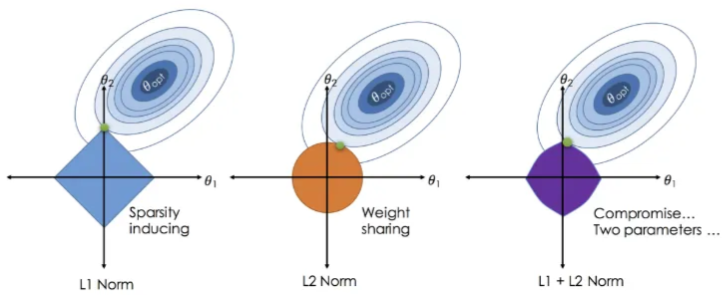
\includegraphics[scale=0.5]{img/regularizers.png}
    \caption{The ridge regularizer draws equipotential circles in our parameter space. The lasso draws a diamond, which tends to give a sparser solution since the loss is most likely to ``touch'' the corners of the contour plots of the regularizer. The elastic net is a linear combination of the ridge and lasso regularizers.} 
    \label{fig:regularizers_visual}
  \end{figure}

  To motivate this even further, let us take the two vectors 
  \begin{align}
    a = \bigg( \frac{1}{\sqrt{d}}, \ldots, \frac{1}{\sqrt{d}} \bigg) \qquad b = ( 1, 0, \ldots, 0)
  \end{align}
  Then the L0, L1, and L2 norms of $a$ are $d, \sqrt{d}, 1$ and those of $b$ are $1, 1, 1$. We want to choose a norm that capture the sparsity of $b$ and distinguishes it from $b$., The L0 norm clearly does this, but the L2 norm does not. The L1 norm is a good compromise between the two. 

  This now raises the question of how to determine a suitable regularization parameter $\lambda$. The next theorem shows a nice concentration property of the Lasso for bounded covariates. 

  \begin{theorem}[Concentration of Lasso]
    Given $(X, Y)$, assume that $|Y| \leq B$ and $\max_j |X_j| \leq B$. Let 
    \begin{equation}
      \beta^\ast = \argmin_{||\beta||_1 \leq L} r(\beta)
    \end{equation}
    be the best sparse linear predictor in the L1 sense, where $r(\beta) = \mathbb{E}[ (Y - \beta^T X)^2]$. Let our lasso estimator be 
    \begin{equation}
      \hat{\beta} = \argmin_{||\beta||_1 \leq L} \hat{r}(\beta) = \argmin_{||\beta||_1 \leq L} \frac{1}{n} \sum_{i=1}^n (Y_i - \beta^T X_i)^2
    \end{equation}
    which minimizes the empirical risk. Then, with probability at least $1 - \delta$, 
    \begin{equation}
      r(\hat{\beta}) \leq r(\beta^\ast) + \sqrt{\frac{16(L+1)^4 B^2}{n} \log \bigg( \frac{\sqrt{2} d}{\sqrt{\delta}} \bigg)} 
    \end{equation}
  \end{theorem}
  \begin{proof}
    
  \end{proof}

  \begin{code}[MWS of Lasso Regression in scikit-learn]
    \noindent\begin{minipage}{.6\textwidth}
    \begin{lstlisting}[]{Code}
      from sklearn.linear_model import Lasso

      X = np.random.randn(10, 5) 
      y = np.random.randn(10)
      # regularization parameter
      model = Lasso(alpha=1e-1)  
      model.fit(X, y) 
      print(model.score(X, y))  
      print(model.intercept_)
      print(model.coef_) 
      print(model.predict(np.array([[1, 2, 3, 4, 5]]))) 
    \end{lstlisting}
    \end{minipage}
    \hfill
    \begin{minipage}{.39\textwidth}
    \begin{lstlisting}[]{Output}
      0.47590269719236045
      -0.8861298412689853
      [0.         0.10767647 0.24172197 0.7427863  0.        ]
      [3.02553422]
      .
      .
      .
      .
      .
    \end{lstlisting}
    \end{minipage}
  \end{code}

  \subsubsection{Soft Thresholding and Proximal Gradient Descent} 

